\documentclass[xcolor={dvipsnames}]{beamer}
\usepackage{color, colortbl}
\usepackage[ngerman,english]{babel}
\usepackage[T1]{fontenc}
\usepackage{lmodern}
\usepackage[compatibility=false]{caption}
\usepackage{subcaption}
\usepackage{tikz}
\usepackage{textgreek}
\usepackage{tabularx}
\usepackage{booktabs}
\usepackage{xspace,multicol}
\usepackage{siunitx}
\usepackage{appendixnumberbeamer}
\usepackage[absolute,overlay]{textpos} %for positioning the logos where I want


\usepackage{animate}
\usepackage{multimedia}
\usepackage{fixltx2e}
\usepackage{multicol}
\usepackage{multirow}
\usepackage{comment}
\DeclareSIUnit\year{yr}
\DeclareSIUnit\micron{\micro\metre}
\DeclareSIUnit\mrad{\milli\rad}
\DeclareSIUnit\gauss{G}
\DeclareSIUnit\nb{\nano\barn}
\DeclareSIUnit\pb{\pico\barn}
\DeclareSIUnit\fb{\femto\barn}

\newcommand{\electron}{e$^-$\xspace}
\newcommand{\positron}{e$^+$\xspace}
\newcommand{\murm}{%
  \ifmmode
    \mathchoice
        {\hbox{\normalsize\textmu}}
        {\hbox{\normalsize\textmu}}
        {\hbox{\scriptsize\textmu}}
        {\hbox{\tiny\textmu}}%
  \else
    \textmu
  \fi
}

\mode<presentation>
{
  \usetheme{CambridgeUS}     
  \usecolortheme{lily} 
  \definecolor{beamer@violet}{rgb}{0.5,0.3,0.5} % changed this
  \setbeamercolor{structure}{fg=beamer@violet!70!cyan}
  \setbeamercolor{palette primary}{fg=black, bg=gray!30!white!50!cyan!20!}
  \setbeamercolor{palette secondary}{fg=black, bg=gray!30!white!30!cyan!40!}
  \setbeamercolor*{palette tertiary}{bg=gray!20!white!20!cyan!60!}
  
  \setbeamercolor{frametitle}{fg=cyan!60!white!40!,bg=cyan!80!black}
  \setbeamercolor{title}{fg=cyan!80!black}
  \setbeamercolor{normal text}{fg=black,bg=white}
  \setbeamercolor{alerted text}{fg=beamer@violet}
  \setbeamercolor{example text}{fg=beamer@violet!70!cyan}
  
  \usefonttheme{structureitalicserif} 
  \setbeamertemplate{navigation symbols}{}
  \setbeamertemplate{caption}[numbered]
}
\newcommand{\sidlogo}{
  \setlength{\TPHorizModule}{1pt}
  \setlength{\TPVertModule}{1pt}
   % textblock{}{x,y}: pos(x) = rightUpperCorner + (x * \TPHorizModule), pos(y) = leftUpperCorner - (y * \TPVertModule)
  \begin{textblock}{1}(323,12)
   
\includegraphics[width=40pt,height=26pt]{figures/SiD.jpeg}
  \end{textblock}
  } 
\newcommand{\ilclogo}{
  \setlength{\TPHorizModule}{1pt}
  \setlength{\TPVertModule}{1pt}
   % textblock{}{x,y}: pos(x) = rightUpperCorner + (x * \TPHorizModule), pos(y) = leftUpperCorner - (y * \TPVertModule)
  \begin{textblock}{1}(323,12)
   
\includegraphics[width=40pt,height=26pt]{figures/ILC.jpeg}
  \end{textblock}
} 
\newcommand{\flukalogo}{
  \setlength{\TPHorizModule}{1pt}
  \setlength{\TPVertModule}{1pt}
   % textblock{}{x,y}: pos(x) = rightUpperCorner + (x * \TPHorizModule), pos(y) = leftUpperCorner - (y * \TPVertModule)
  \begin{textblock}{1}(315,12)
   
\includegraphics[width=60pt,height=26pt]{figures/fluka_logo.png}
  \end{textblock}
} 

\title[ILC250 backgrounds \& SiD Occupancy]{\textbf{\alert{LCWS2017, Strasbourg} \\ \vspace*{0.5cm}  Background \& SiD Occupancy Studies\\for the ILC250 stage}}
\author{\textbf{Anne Sch\"utz}}
\institute{\textbf{DESY}}
\date{\textbf{24. October 2017}}

\titlegraphic{\hspace*{1cm}
\includegraphics[height=1.0cm]{figures/ILC.jpeg}\hfill~%
   
\includegraphics[height=1.0cm]{figures/DESY_Logo.png}\hspace*{1.5cm}
}

\begin{document}

{
\usebackgroundtemplate{
 \tikz\node[opacity=0.1]{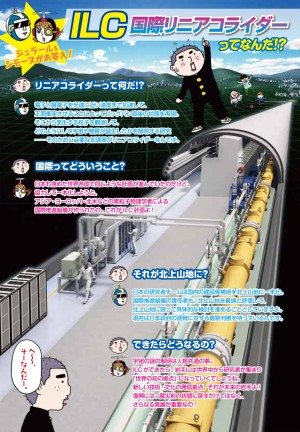
\includegraphics[width=\paperwidth]{figures/Iwatecomics.jpg}};
 % \tikz\node[opacity=0.2]{\centering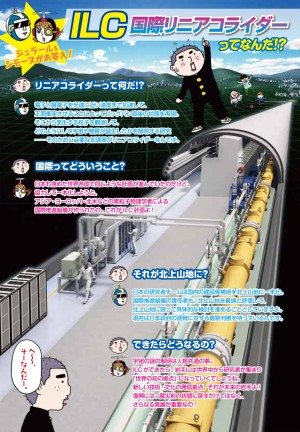
\includegraphics[height=\paperheight]{figures/Iwatecomics.jpg}};
 }
\begin{frame}
  \titlepage
\end{frame}
}
\setcounter{tocdepth}{2}
\begin{frame}{Table of contents}
  \tableofcontents
\end{frame}

%---------------------------------------------------------------------------------------------------------

\setcounter{tocdepth}{3}
\AtBeginSubsection[] {
  \begin{frame}<beamer>
     \tableofcontents[currentsection,
     currentsubsection,
     %hideothersubsections,
     subsectionstyle=show/shaded/hide,
     subsubsectionstyle=show/show/hide]
  \end{frame}
}

%--------------------------------------------------------------------------------------------------------------


%--------------------------------------------------------------------------------------------------------------
\AtBeginSection[] {
  \begin{frame}<beamer>
     \tableofcontents[currentsection,
     currentsubsection,
     %hideothersubsections,
     subsectionstyle=show/shaded/hide,
     subsubsectionstyle=show/show/hide]
  \end{frame}
}

\section{New beam parameter sets for the ILC250 stage}

\begin{frame}{ILC250 Beam Parameter Sets}
 \begin{table}
\caption{Possible beam parameter sets for the ILC250 stage.\\{\small The table only lists the parameters that are to be changed with respect to the original ILC250 parameters given in the Technical Design Report (TDR)~\cite[p. 11]{TDR1}.}}
\label{tab:Parameters}
\centering
\begin{tabularx}{0.55\textwidth}{llll}
\hline\hline
\textbf{Set}  & \textbf{$\epsilon_x$ [\murm m]} & \textbf{$\beta_x$ [mm]} & \textbf{$\beta_y$ [mm]}\\
\hline
\cline{1-4}
\hline
 TDR & 10 & 13.0 & 0.41\\
 (A) & 5 & 13.0 & 0.41\\
 (B) & 5 & 9.19 & 0.41\\
 (C) & 5 & 9.19 & 0.58\\
\hline\hline
\end{tabularx}
\end{table}
\alert{Reduced emittance leads to stronger beam-beam interactions, and therefore to increased \positron \electron pair background.}
\end{frame}

\section{Pair background density}
\begin{frame}{Background event generation using GuineaPig}
 The background generation in GuineaPig \textit{does not include a crossing angle}!\\
 The crossing angle is applied later on in the Geant4 simulation of the SiD detector.
\end{frame}

\begin{frame}{Pair background density in a 5\,T solenoid field}
\sidlogo
 \begin{figure}
\centering
\begin{subfigure}[t]{0.35\textwidth}
\centering
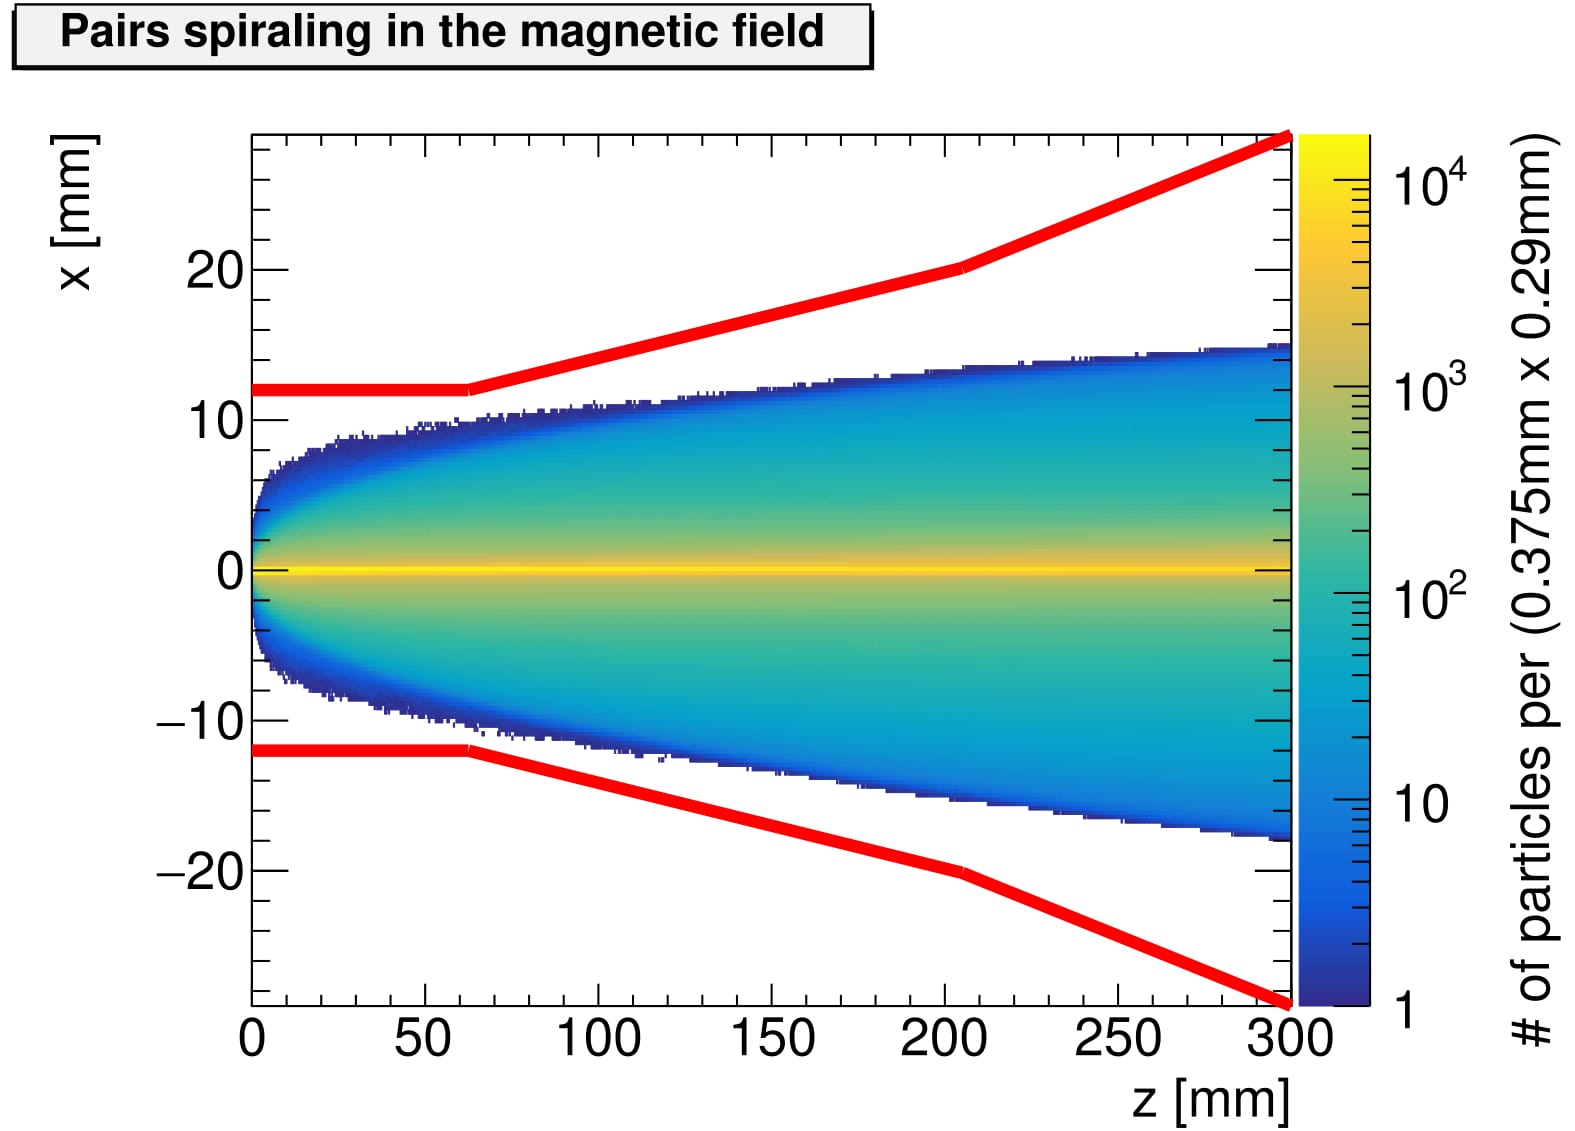
\includegraphics[width=\textwidth]{ILC250_figures/Helix_tracks_xz_100bunches_250GeV_5T_DanielJeans-1.jpg}
\caption{ILC250 set (TDR)}
\end{subfigure}
\hspace*{0.1cm}
\begin{subfigure}[t]{0.35\textwidth}
\centering
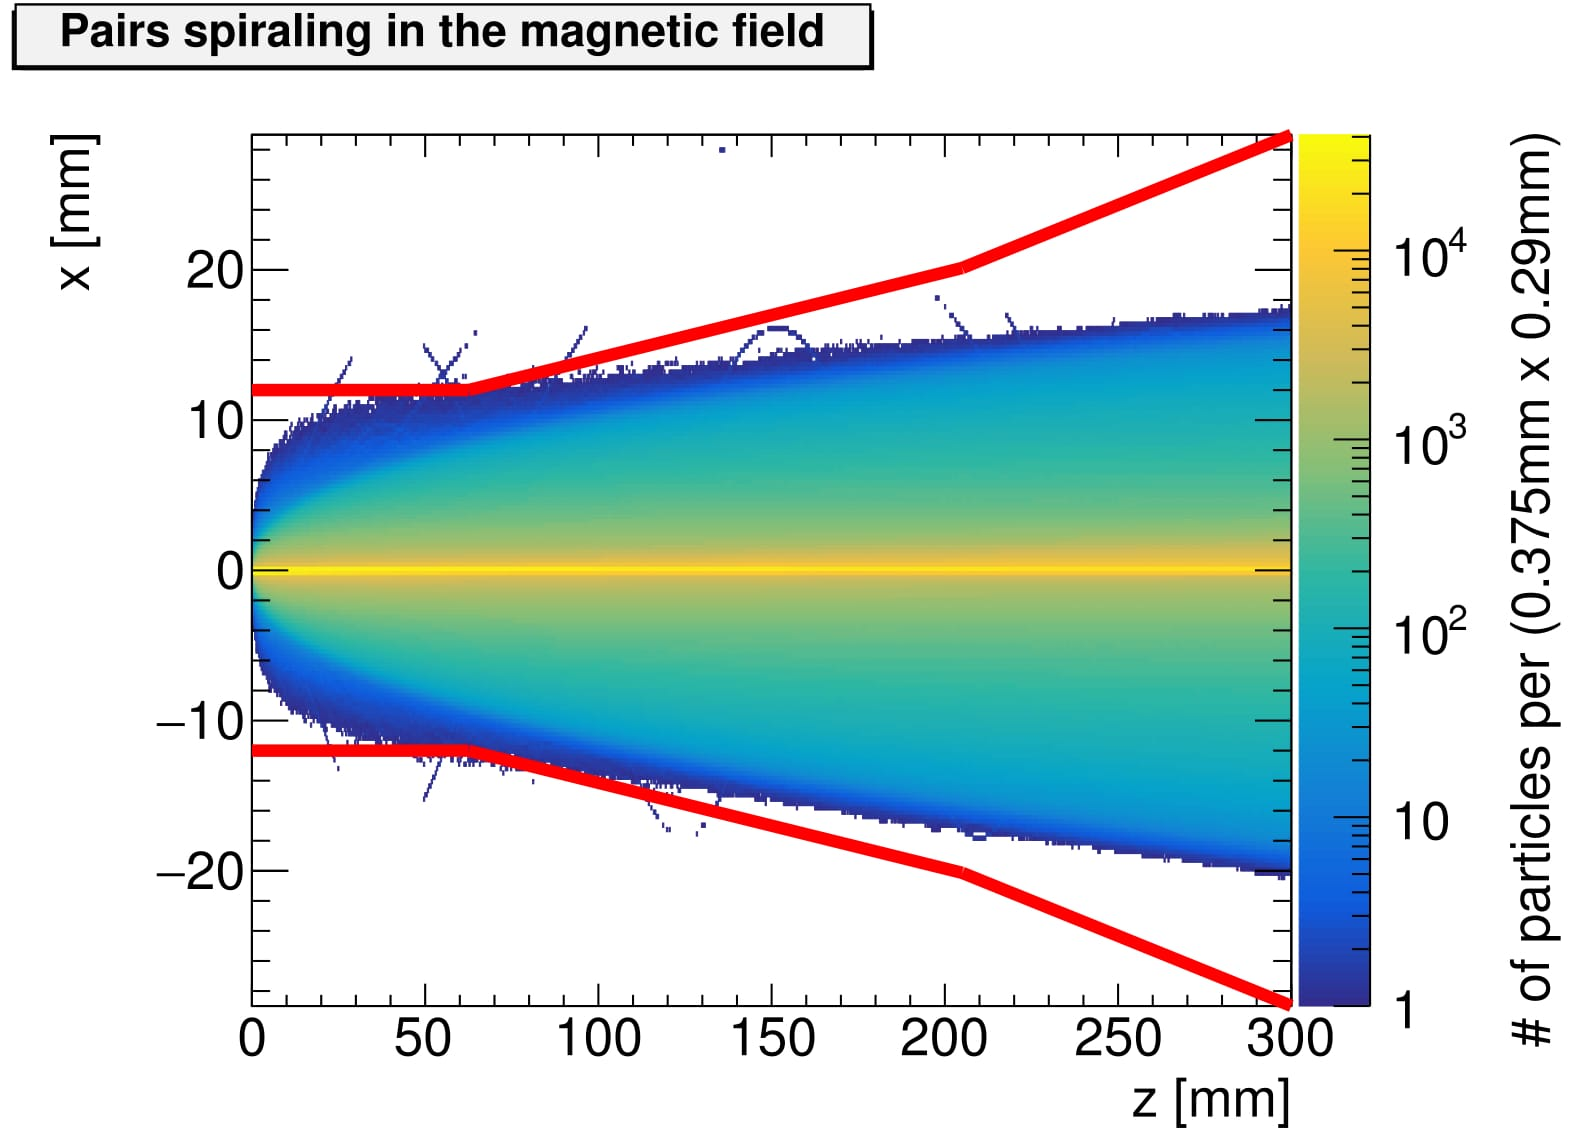
\includegraphics[width=\textwidth]{ILC250_figures/Helix_tracks_xz_80bunches_250GeV_5T_Reduced_Emittance_x-1.jpg}
\caption{ILC250 set (A)}
\end{subfigure}
\\
\begin{subfigure}[t]{0.35\textwidth}
\centering
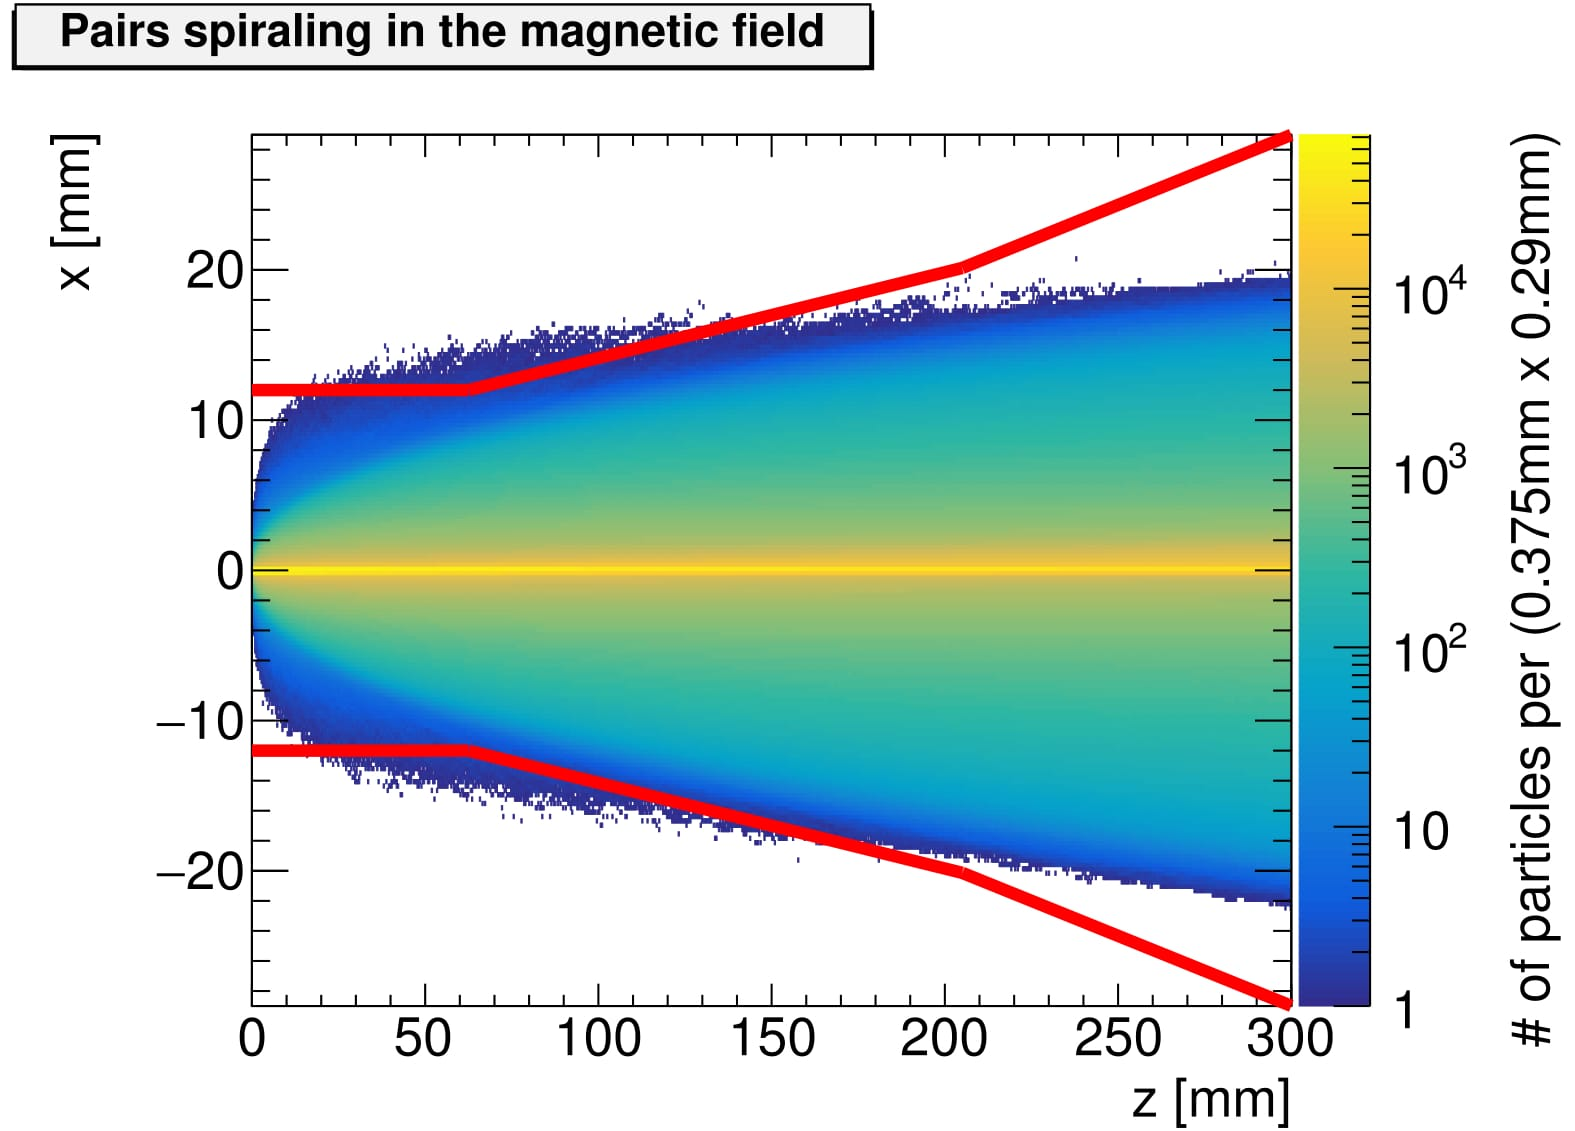
\includegraphics[width=\textwidth]{ILC250_figures/Helix_tracks_xz_50bunches_250GeV_5T_Reduced_Emittance_x_Reduced_Beta_x-1.jpg}
\caption{ILC250 set (B)}
\end{subfigure}
\hspace*{0.1cm}
\begin{subfigure}[t]{0.35\textwidth}
\centering
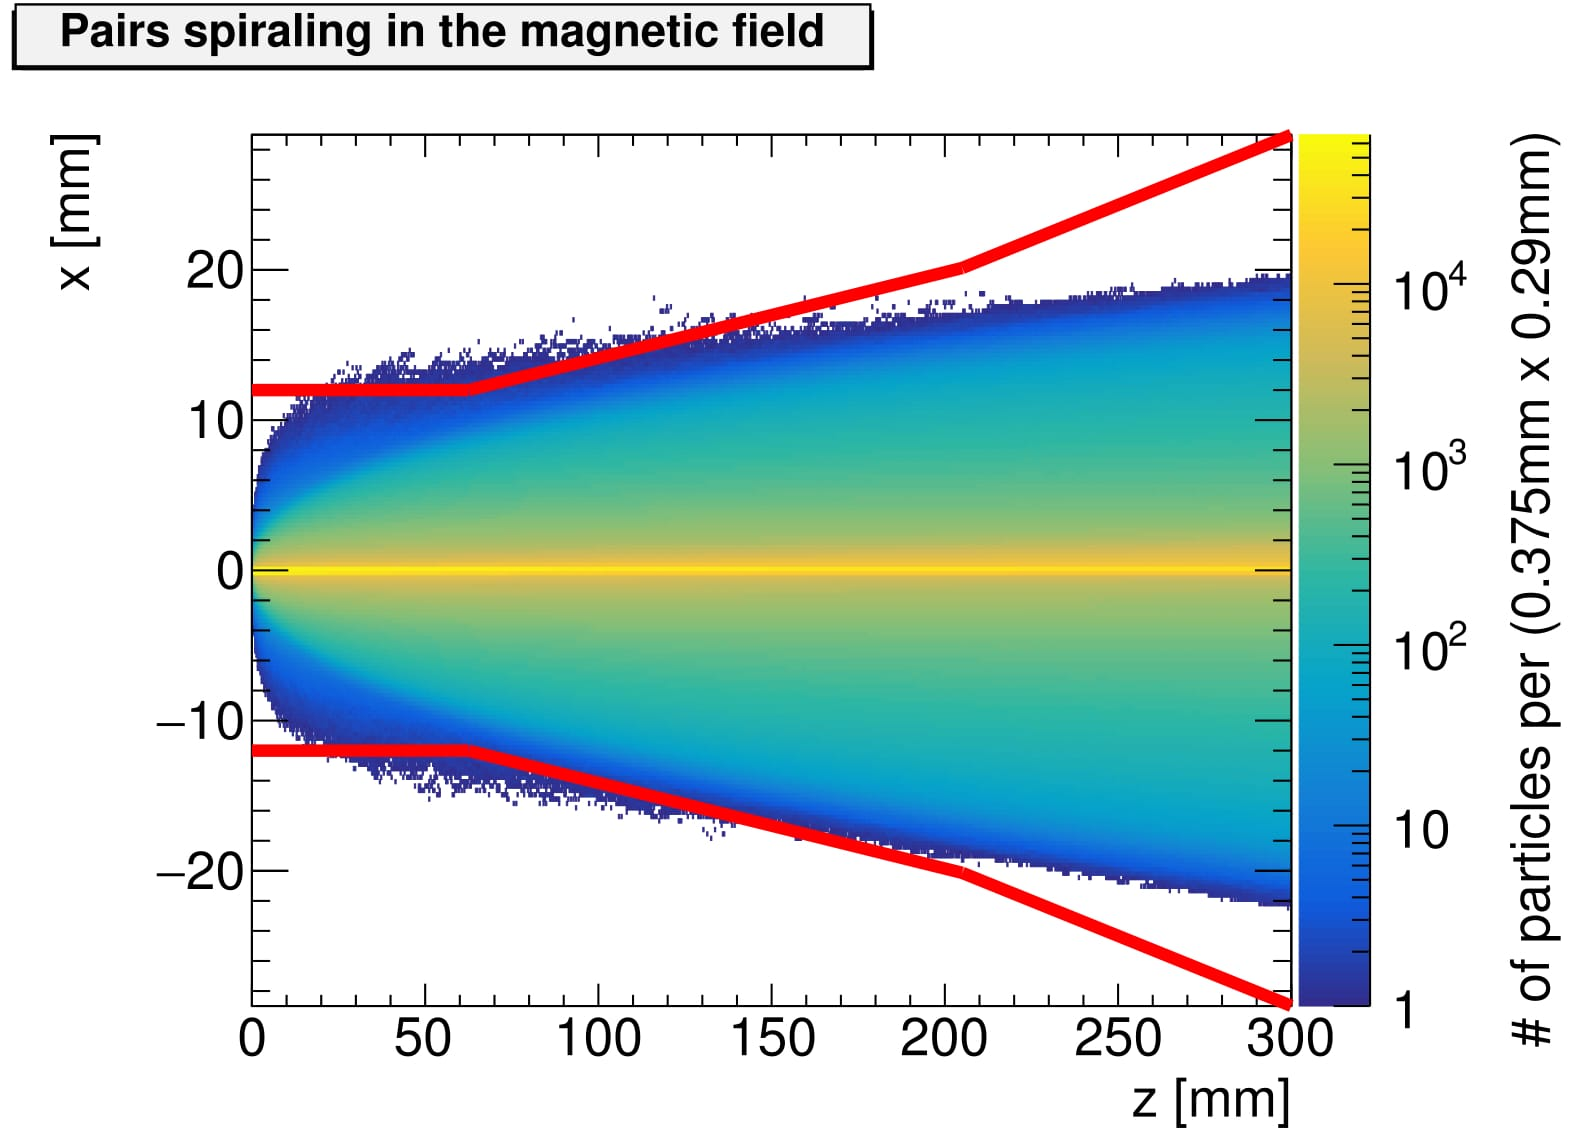
\includegraphics[width=\textwidth]{ILC250_figures/Helix_tracks_xz_50bunches_250GeV_5T_Reduced_Emittance_x_Reduced_Beta_x_Increased_Beta_y-1.jpg}
\caption{ILC250 set (C)}
\end{subfigure}
\caption{Pair background density for the different ILC250 beam parameter sets.
The beam pipe is represented by the red solid lines.}
\label{fig:Envelopes}
\end{figure}

\end{frame}

\begin{frame}{Projection of the pair background density along x}
\sidlogo
\begin{center}
 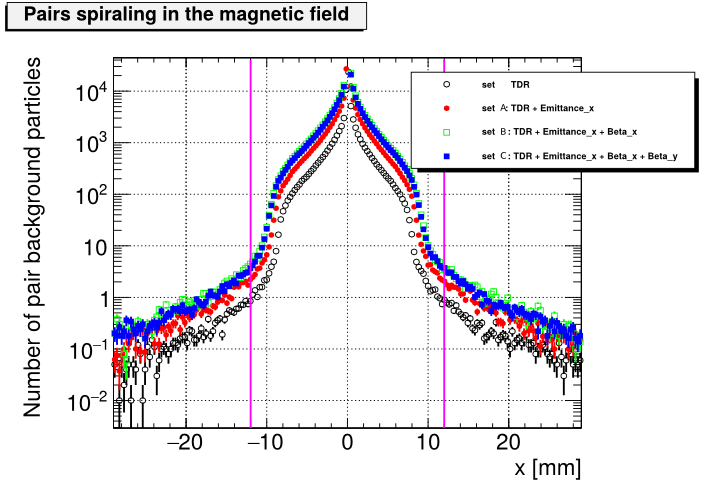
\includegraphics[width=0.72\textwidth]{ILC250_figures/HelixEnvelope_Projection_Comparison_250GeV_parametersets_NEWSETNAMES.png}
\end{center}
The envelopes are in all schemes well contained within the beam pipe. Less than 10 particles per bunch crossing are to be expected outside the beam pipe.
\end{frame}

\section{SiD Occupancy}
\begin{frame}{SiD Vertex Detector Occupancy: All layers}
\sidlogo
 \begin{figure}
\centering
\begin{subfigure}[t]{0.48\textwidth}
\centering
\includegraphics[width=\textwidth]{ILC250_figures/Occupancy_Comparison_All_layers_wrt__cells_ILC250_ALL_SETS_6Sep2017_NEWSETNAMES.png}
\caption{\alert{Normalized Occupancy}: Number of cells containing a certain amount of hits, normalized by the total number of cells of the vertex detector.}
\end{subfigure}
\hspace*{0.2cm}
\begin{subfigure}[t]{0.48\textwidth}
\centering
\includegraphics[width=\textwidth]{ILC250_figures/Occupancy_Comparison_All_layers_deadcells_ILC250_ALL_SETS_6Sep2017_NEWSETNAMES.png}
\caption{\alert{Normalized number of dead cells}: Number of cells with full buffer, normalized by the total number of cells of the vertex detector.}
\end{subfigure}
\end{figure}
\end{frame}

\begin{frame}{SiD Vertex Detector Occupancy: Layer 0}
\sidlogo
\begin{center}
 \includegraphics[width=0.6\textwidth]{ILC250_figures/Occupancy_Comparison_Layer_0_numcells_ILC250_ALL_SETS_6Sep2017_NEWSETNAMES.png}
\end{center}
The occupancy in layer 0 for the new sets is significantly increased with respect to the TDR scheme.
\end{frame}

\section{Conclusion}
\begin{frame}
\sidlogo
 According to the shown studies of the background density and the SiD occupancy for the new ILC250 parameter sets, SiD is confident that the increased occupancy can be accommodated in the design of the Vertex Detector.\\
 The SiD Optimization Group gives green light for the current Change Request, and welcomes the efforts on increasing the luminosity for the ILC250 stage.
\end{frame}


%---------------------------------------------------------------------------------

\section*{The end}
{
\usebackgroundtemplate{
 \tikz\node[opacity=0.1]{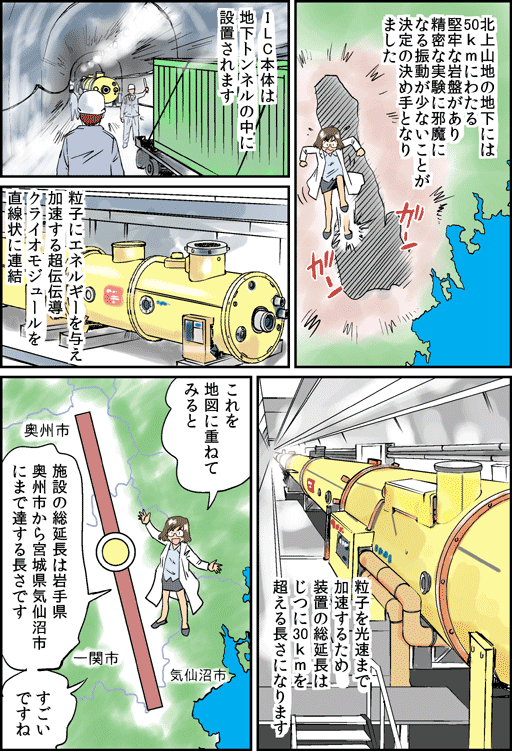
\includegraphics[width=\paperwidth,resolution=200]{figures/ilc-Comic.png}};
 % \tikz\node[opacity=0.2]{\centering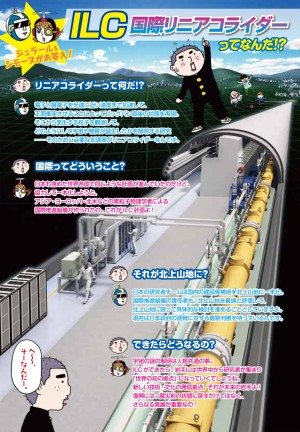
\includegraphics[height=\paperheight]{figures/Iwatecomics.jpg}};
 }
\begin{frame}
\ilclogo
\begin{center}
\textcolor{RubineRed}{
	\LARGE Thanks!\\
}
\end{center}
\end{frame}
}

\section*{References}
\begin{thebibliography}{9}
\setbeamertemplate{bibliography item}[text]
\begin{frame}{References for the Pair background study}
\tiny
\bibitem{AWLC_Yokoya}
\bibitem{AWLC_Jeans}
\bibitem{TDR1} T. Behnke, et al., \emph{The International Linear Collider - Technical Design Report, Volume 1}, 2013.
\end{frame}
\end{thebibliography}

%--------------------------------------------------------------------------------
\appendix

\begin{frame}
\begin{center}
\LARGE Additional Material
\end{center}
  \tableofcontents
\end{frame}

\section{ILC}

\subsection{The ILC beam parameters}
\begin{frame}{ILC baseline parameters}
\ilclogo
\begin{center}
	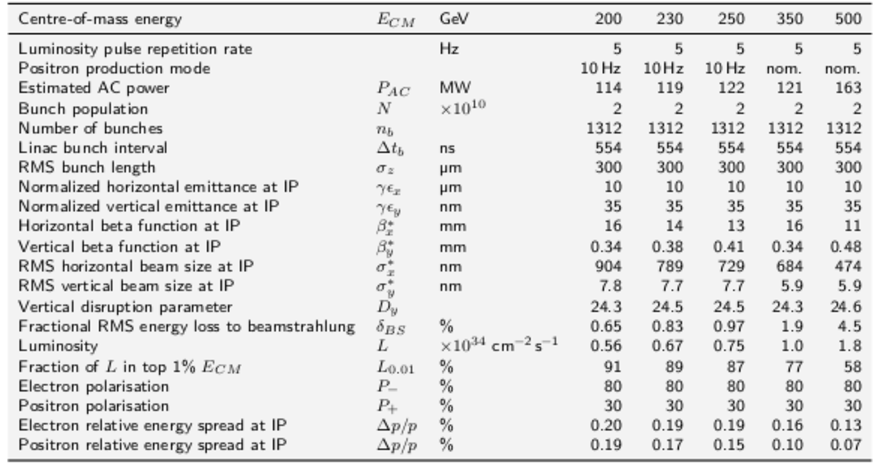
\includegraphics[width=\textwidth]{figures/ILCTDR-VOLUME_3-PART_II_ILCparameters.pdf}
\end{center}
\end{frame}
\begin{frame}{ILC parameters for the different upgrade stages}
\ilclogo
\begin{center}
	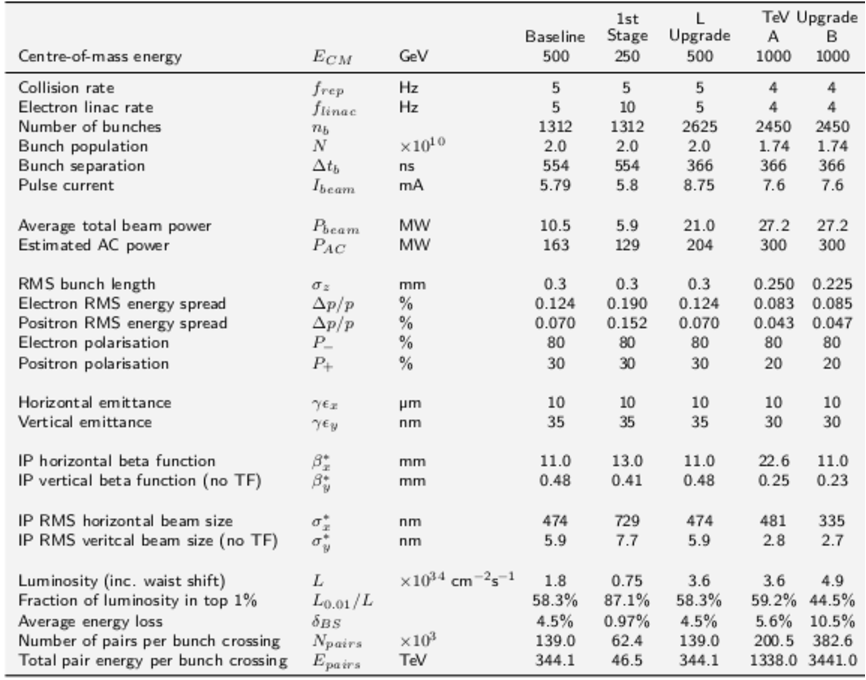
\includegraphics[width=0.8\textwidth]{figures/ILCTDR-VOLUME_3-PART_II_ILCparametersUpgrades.pdf}
\end{center}
\end{frame}

\end{document}
